\documentclass{beamer}
%\usetheme{Madrid}
%\usetheme{Boadilla}
%\usetheme{default}
%\usetheme{Warsaw}
%\usetheme{Bergen}
%\usetheme{Frankfurt}
\usetheme{Darmstadt}

%\usecolortheme{seahorse}
%\usecolortheme{beaver}
\usecolortheme[named=orange]{structure}

\setbeamertemplate{footline}[page number]
%\setbeamercovered{transparent}
\setbeamercovered{invisible}
\setbeamertemplate{navigation symbols}{}

\usepackage{multimedia}
\usepackage{graphicx}
\usepackage[utf8]{inputenc}
%\usepackage[T1]{fontenc}
\usepackage[frenchb]{babel} 
\usepackage[all]{xy}
\usepackage{multirow}
\usepackage{lmodern}
\usepackage{subfigure}
\usepackage{ulem}
\usepackage{hyperref}

\usepackage[backend=bibtex]{biblatex}
\addbibresource{papers.bib}

\setbeamertemplate{caption}[numbered] 

%% --------------

\title{Cartographie, localisation et navigation muti-robots utilisant la vision omnidirectionnelle}
\subtitle{Soutenance de Projet de Fin d'\'Etudes}
\author{L\'eo \textsc{Baudouin}\\\emph{leo.baudouin@ifma.fr}}
\institute{
  Institut Pascal (LASMEA)
}
\date{20 septembre 2012}

%% --------------

\begin{document}

\begin{frame}
  \titlepage
  \begin{tabular}{c c c c c}
    \begin{minipage}{0.2\linewidth}
      
\includegraphics[height=10mm]{images/EU.jpg}
    \end{minipage}
    &
    \begin{minipage}{0.2\linewidth}
      
\includegraphics[height=10mm]{images/auvergne.png}
    \end{minipage}
    &
    \begin{minipage}{0.12\linewidth}
      
\includegraphics[height=10mm]{images/logo-IFMA.jpg}
    \end{minipage}
    &
    \begin{minipage}{0.2\linewidth}
      
\includegraphics[height=6mm]{images/logo-LASMEA}
    \end{minipage}
    &
    \begin{minipage}{0.2\linewidth}
      
\includegraphics[height=10mm]{images/logo-IP}
    \end{minipage}
  \end{tabular}
\end{frame}


\begin{frame}{Plan}
  \tableofcontents
\end{frame}

%% --------------

\section{Introduction}
\subsection*{Laboratoire}

\begin{frame}{Institut Pascal}
  \begin{tabular}{l l}
    \begin{minipage}{0.3\linewidth}
      
\includegraphics[width=\linewidth]{images/logo-IP.jpg}
    \end{minipage}
    &
    \begin{minipage}{0.8\linewidth}
      Le laboratoire de l'Institut Pascal est composé de trois équipes regroupant au total une centaine de chercheurs.
      \begin{itemize}
      \item ComSee
      \item Rosace
      \item ???
      \end{itemize}
    \end{minipage}
  \end{tabular}

\end{frame}


\begin{frame}
  Page 2
\end{frame}

\subsection*{Robotique autonome}

\begin{frame}
  Google Car
\end{frame}

\begin{frame}
  Volvo
\end{frame}

\subsection*{Thèse}

\begin{frame}{Projet de thèse}
  Page 1
\end{frame}

\begin{frame}
  Page 2
\end{frame}

%% --------------

\section{Recherche}
\subsection*{Méthodes}

\begin{frame}{Recherche bibliographique}
  Comment chercher ?
  Comment trouver ?
  Disponibilité ?
  Achats ?
  Aller de publi en publi...
  Trouver des vidéos sur le net ...
  Site web ...
  Notions de maths dans les thèses
\end{frame}

\subsection*{Articles}

\begin{frame}{Exemple}
%Auteurs, écriture, publication (tro, iros, \dots)

Article :\\
\begin{scriptsize}
\mbox{
\citeauthor{baudouin:humanoids:11}
\citetitle{baudouin:humanoids:11}
\cite{baudouin:humanoids:11}
}
\end{scriptsize}
%\vspace{5mm}

Thèse :\\
\begin{scriptsize}
\mbox{
\citeauthor{Courbon09PhD}
\citetitle{Courbon09PhD}
\cite{Courbon09PhD}}
\end{scriptsize}
\vspace{5mm}


Exemple :\\
%\begin{tiny}
\begin{scriptsize}
@inproceedings\{baudouin:humanoids:11,\\
	\hspace{5mm} author = "L. Baudouin and N. Perrin and T. Moulard and F. Lamiraux and O. Stasse and E. Yoshida",\\
	\hspace{5mm} booktitle = "\{IEEE/RAS International Conference on Humanoid Robotics (Humanoids'11)\}",\\
	\hspace{5mm} title = "\{Real-time Replanning Using 3D Environment for Humanoid Robot\}",\\
	\hspace{5mm} url = "http://ubuntuone.com/6zyz487WVECpyW88tEfQz5",\\
	\hspace{5mm} year = "2011"\\
\}
\end{scriptsize}
%\end{tiny}

\end{frame}

\begin{frame}{Bibliographie}
%\begin{minipage}{0.5\linewidth}
\printbibliography
%\end{minipage}
\end{frame}


\subsection*{Gestion Bibliographique}

\begin{frame}{Bibliographie}
  80 ouvrages, image de KBibTex, exemples, but, intérêts, reconnaissance
\end{frame}

\begin{frame}
\begin{figure}
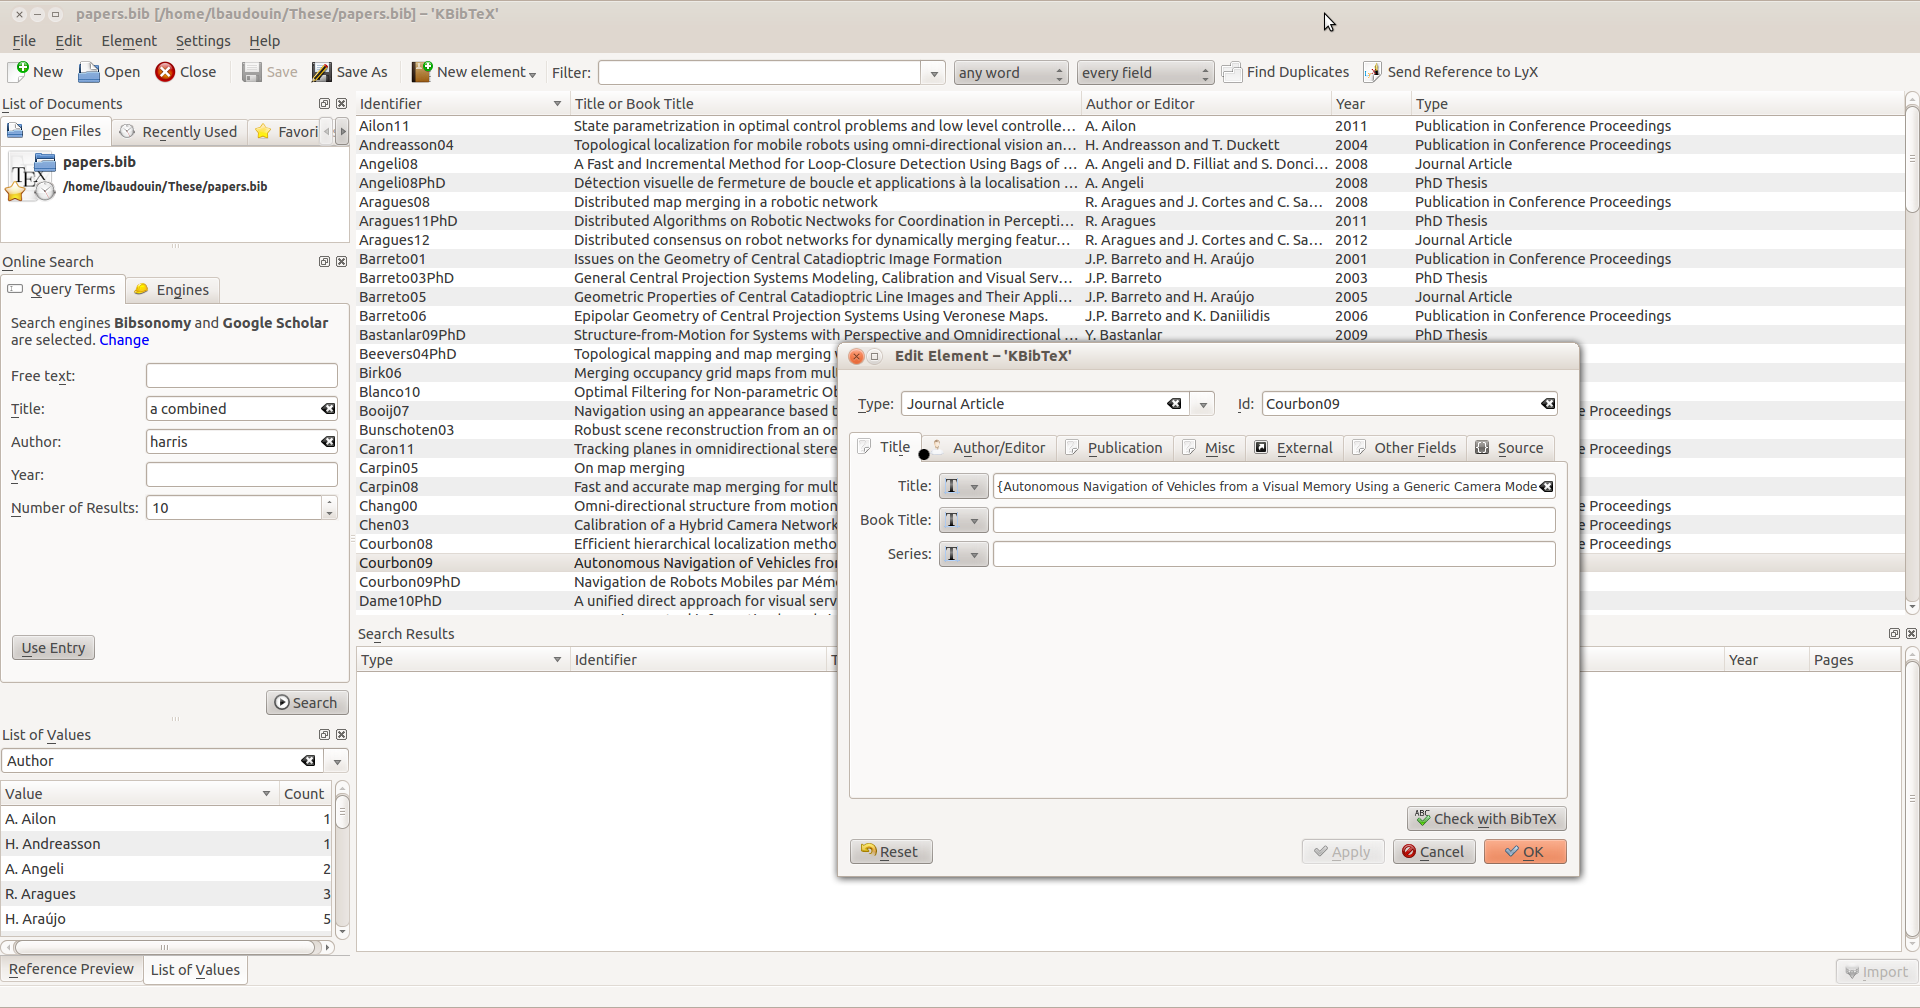
\includegraphics[width=1.0\linewidth]{images/KBibTex.png}
\caption{Capture d'écran de KBibTex, ligiciel libre de gestion de bibliographie}
\end{figure}
\end{frame}

%% --------------

\section{Avancement}

\subsection*{Vision}
\begin{frame}{Reconstruction 3D}
  Vidéo du programme\\
  Erreurs
\end{frame}

\subsection*{Création de cartes}
\begin{frame}{Développement}
  Sovin, loop\_closure, SSBA, robotvision
\end{frame}

\subsection*{Navigation}
\begin{frame}

\end{frame}

\subsection*{Situation}
\begin{frame}
Retard
\end{frame}

%% --------------

\section{Conclusion}
\subsection*{Suite des travaux}
\begin{frame}{}
  \begin{itemize}
  \item 123
  \item 456
  \end{itemize}
\end{frame}

\subsection*{Première Conclusion}
\begin{frame}{Conclusion}

\end{frame}


\end{document}  
